\documentclass[hidelinks]{article}
\usepackage[utf8]{inputenc}
\usepackage[T1]{fontenc}
\usepackage[margin=1in]{geometry}
\usepackage{amsmath,caption,color,enumitem,float,graphicx,hyperref,lipsum,multicol,quoting,soul,tabularx}
\title{Analyzing Movies Using Phrase Mining}
\author{Daniel Lee \and Huilai Miao \and Yuxuan Fan}

\begin{document}
\maketitle

\begin{abstract}
Movies often capture human culture and major events across time. As a result, movies are an unconventional but rich source of human history from which we can derive insight. Previous work addresses either a textual analysis of movie plots or the use of phrase mining for natural language processing, but not both. Here, we propose a novel analysis of movie plots by extracting key phrases from movie plot summaries using AutoPhrase, a phrase mining framework. Using these phrases, we analyze movies through 1) an exploratory data analysis that examines the progression of human culture over time, 2) the development and interpretation of a classification model that predicts movie genre, and 3) the development and interpretation of a clustering model that clusters movies. This application of phrase mining to movie plots provides results consistent with human history and provides a unique perspective in understanding human culture.
\end{abstract}

\begin{multicols}{2}
\section{Introduction}
Movies often capture human culture and major events across time. We can learn from this rich source of human history through a comprehensive textual analysis of movies, i.e., movie plot summaries.

Here, we propose an analysis of movie plots by extracting key phrases corresponding to discrete entities of human culture and events. Such an analysis can help us better understand change of popular topics, public attitudes, major themes, and the overall progression of human culture throughout history.

This analysis is novel since we extract history from movie plots, an unconventional source, instead of relying on historical texts directly; we expect such a study to provide a unique perspective as a result. In addition, we expect such a study to be especially useful for history non-experts, as we extract key phrases that provide relevant keywords for further research by the reader.

Previous work addresses either a textual analysis of movie plots or the use of phrase mining for natural language processing, but not both. Previous analyses of movies are limited as they tend to use extract n-grams using raw frequencies instead of a sophisticated phrase mining framework such as \href{https://github.com/shangjingbo1226/AutoPhrase}{AutoPhrase} \cite{DBLP:journals/corr/ShangLJRVH17}. Here, we explore a novel approach by applying phrase mining to the analysis of movies plots.

\section{Data}
Our dataset comes from the \href{http://www.cs.cmu.edu/~ark/personas/}{CMU Movie Summary Corpus} \cite{Bamman2013LearningLP} and consists of movie plot summaries extracted from Wikipedia and movie metadata extracted from Freebase.

The dataset consists of around 42,000 movies from 1893 to 2014 as seen in Figure \ref{figure:number_movies_per_year_bar_chart}, a sizable dataset for our study. Table \ref{table:variables} describes the variables of the processed dataset. Although movies can come from different countries and may be in different languages, all of the movie plot summaries are in English (as the dataset is extracted from English Wikipedia).

The variable of focus here is \texttt{summary}, from which we extract key phrases to drive our analysis.

\begin{figure*}
\caption{Number of movies in the dataset}
\centering
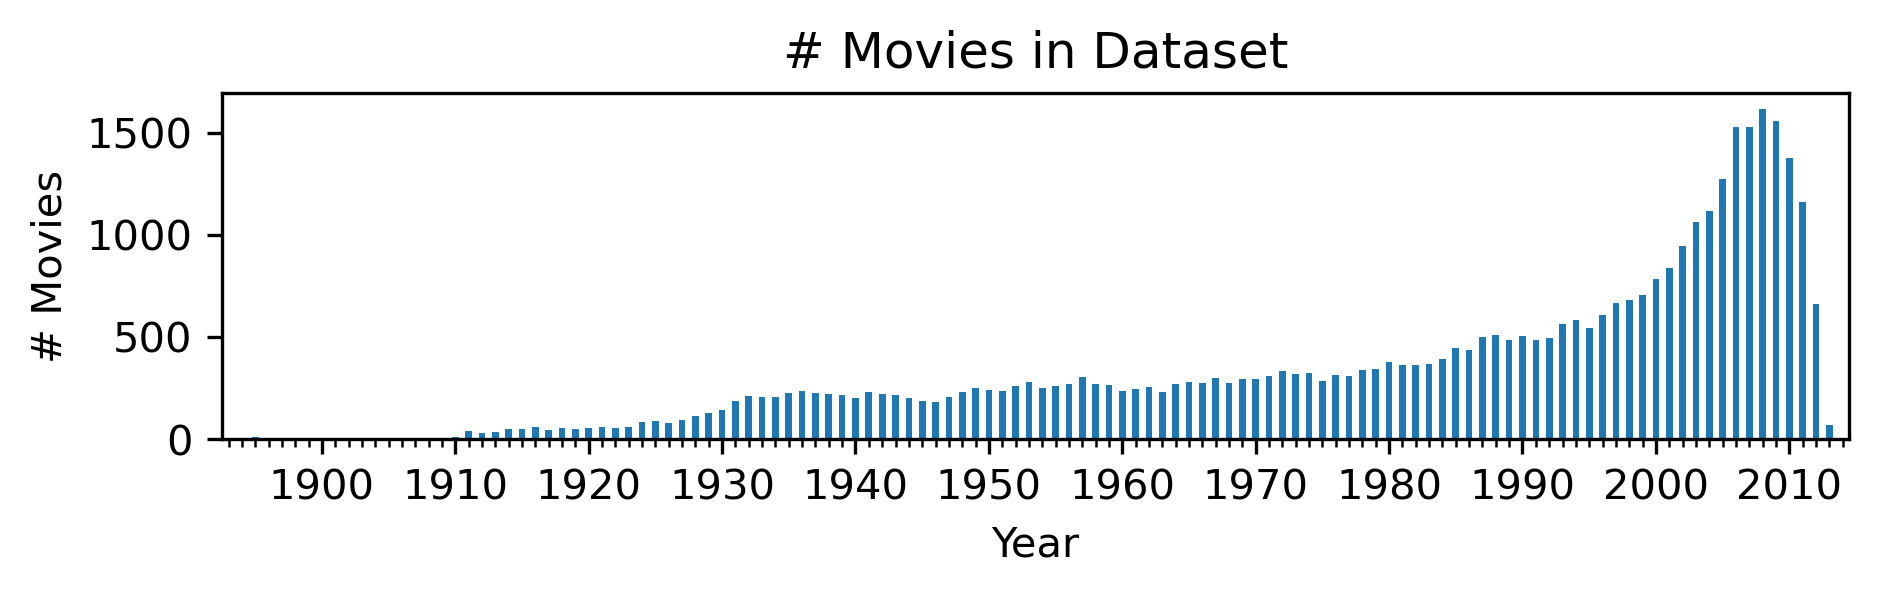
\includegraphics[width=5in]{figures/number_movies_per_year_bar_chart.png}
\label{figure:number_movies_per_year_bar_chart}
\end{figure*}

\begin{table*}
\caption{Dataset variables}
\centering
\begin{tabularx}{.8\textwidth}{llX}
    \textbf{Variable} & \textbf{Description} & \textbf{Example} \\
    \hline
    \texttt{name} & Movie name & \textit{Star Wars Episode IV: A New Hope} \\
    \texttt{date} & Movie release date & \textit{1977-05-25} \\
    \texttt{revenue} & Movie box office revenue (USD) & \textit{775,398,007} \\
    \texttt{runtime} & Movie runtime (minutes) & \textit{122} \\
    \texttt{languages} & Movie languages & \textit{\{English\}} \\
    \texttt{countries} & Movie countries & \textit{\{United States of America\}} \\
    \texttt{genres} & Movie genres & \textit{\{Action, Adventure, Coming-of-age, Family, Fantasy, Science Fiction, Space western\}} \\
    \texttt{summary} & Movie plot summary & \textit{The film begins with an opening crawl explaining that the galaxy is in a state of civil war and that spies for the Rebel Alliance have \ldots} \\
\end{tabularx}
\label{table:variables}
\end{table*}

\section{Methods}
We first extract key phrases from \texttt{summary} using AutoPhrase \cite{DBLP:journals/corr/ShangLJRVH17}, a sophisticated phrase mining framework that extracts high-quality phrases from a given text corpus. We use AutoPhrase due to its ability to extract high-quality phrases more effectively than traditional, rudimentary, phrase mining techniques, while maintaining minimal human effort during training.

We first train AutoPhrase on all movie plot summaries in the dataset, then extract the key phrases from each individual summary and add these phrases as a variable in our dataset as seen in Table \ref{table:additional_variables}. Figure \ref{figure:key_phrases_example} gives an example of phrases extracted from a movie plot summary by AutoPhrase. Nearly all extracted phrases are indeed high-quality and describe ideas, events, objects, and characters in the movie plot well.

\begin{table*}
\caption{Additional variables}
\centering
\begin{tabularx}{.8\textwidth}{llX}
    \textbf{Variable} & \textbf{Description} & \textbf{Example} \\
    \hline
    \texttt{phrases} & Phrases extracted from \texttt{summary} & \textit{\{alderaan, anakin skywalker, assault, aunt and uncle, bay, c-3po, chewbacca, civil war, commanding officer, darth vader, \ldots\}} \\
\end{tabularx}
\label{table:additional_variables}
\end{table*}

\begin{figure*}
\caption{Example of phrases extracted by AutoPhrase}
\begin{quoting}[leftmargin=.1\textwidth]
\small\textit{The \hl{film} begins with an opening crawl explaining that the \hl{galaxy} is in a \hl{state} of \hl{civil war} and that spies for the \hl{Rebel Alliance} have \hl{stolen} plans to the Galactic Empire's \hl{Death Star}, a \hl{heavily armed} and armored \hl{space station} capable of annihilating an \hl{entire planet}. \hl{Rebel leader} \hl{Princess Leia} is in possession of the plans, but her \hl{ship} is captured by Imperial forces under the command of the evil \hl{lord} \hl{Darth Vader}. Before she is captured, \hl{Leia} hides the plans in the \hl{memory} of an astromech droid called \hl{R2-D2} , along with a holographic \hl{recording}. The small droid flees to the surface of the \hl{desert planet} \hl{Tatooine} with \hl{fellow} protocol droid \hl{C-3PO} . The \hl{droids} are quickly captured by\ldots}
\end{quoting}
\label{figure:key_phrases_example}
\end{figure*}

Our analysis consists of three parts that build off of these extracted phrases:
\begin{enumerate}
    \item An exploratory data analysis (EDA) that examines the progression of human culture over time.
    \item The development and interpretation of a classification model that predicts movie genre.
    \item The development and interpretation of a clustering model that clusters movies.
\end{enumerate}
We expect the combination of these three methods to give us valuable insight into human culture.
\subsection{EDA}
We perform an EDA to discover how human culture and events have evolved throughout time. Here, we use statistical signals, i.e., tf-idf, to identity when certain phrases (ideally corresponding to discrete entities of of human culture and events) are popular and relevant.

We use tf-idf to measure a phrase's relevance in time where each phrase is a term and each period of time (e.g. a year or decade) is a document. We use sublinear term frequency (tf) scaling to reduce the significance of very common phrases (e.g. ``film'', ``life'') that are uninformative in our analysis.

Here, the tf-idf with sublinear tf scaling for a term $t$ of a document $d$ is given by
$$\text{tf-idf}(t, d) = (1 + \log\text{tf}(t, d)) \cdot \left(\log\frac{1 + n}{\text{1 + df}(t)} + 1\right)$$
where $n$ is the total number of documents and $\text{df}(t)$ is the document frequency of $t$.

Given a tf-idf vector for each period of time, we then normalize each tf-idf vector to have a Euclidean norm of 1.
\subsection{Classification}
\subsection{Clustering}

\section{Results}
\subsection{EDA}
\subsection{Classification}
\subsection{Clustering}

\section{Discussion}

\bibliographystyle{plain}
\nocite{10.1145/2723372.2751523}
\bibliography{report}

\section{Appendix}
\begin{figure*}
\caption{Top phrases by year}
\centering
% 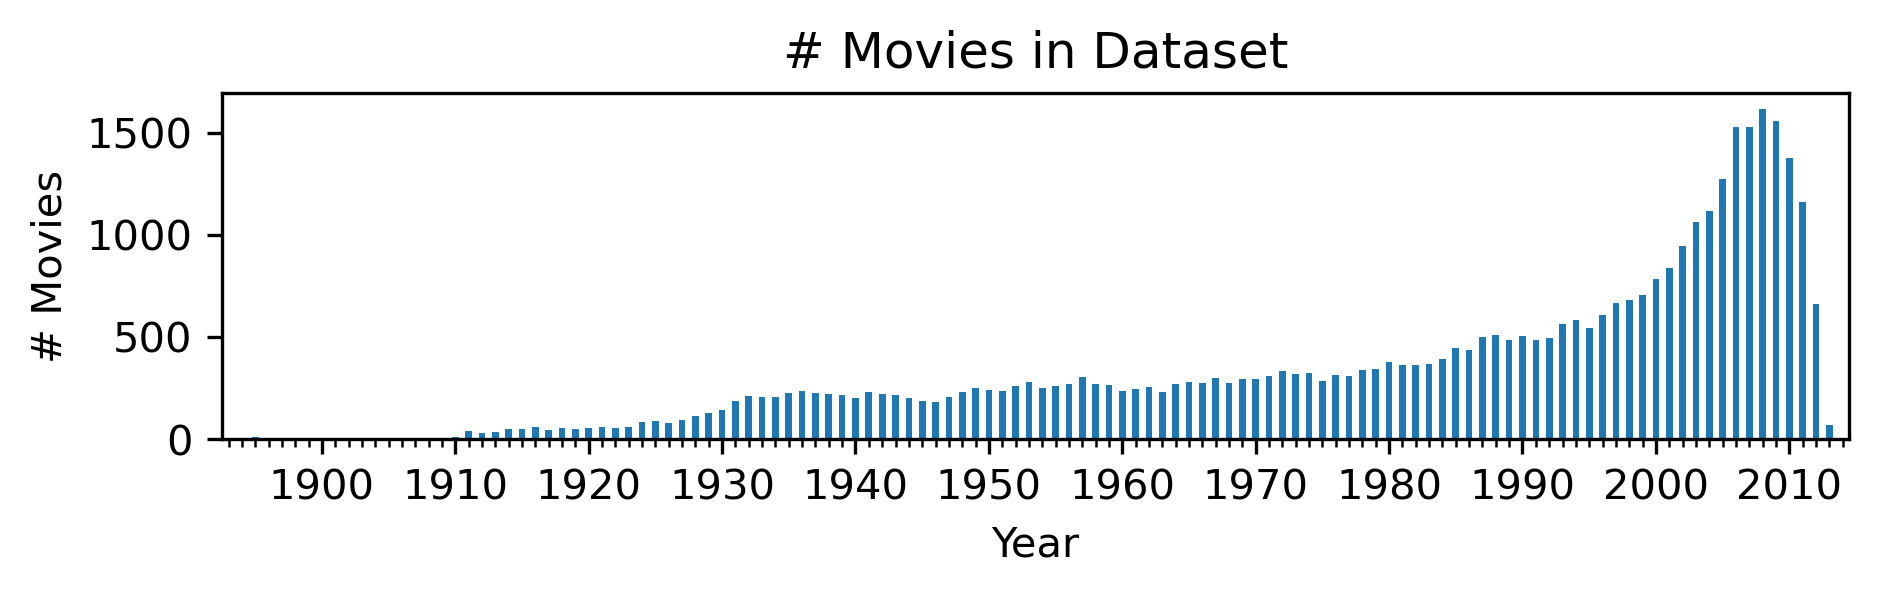
\includegraphics{figures/number_movies_per_year_bar_chart.png}
\label{figure:top_phrases_by_year}
\end{figure*}
\end{multicols}

\end{document}
